\documentclass[12pt,a4paper,oneside]{article}

%\usepackage[utf8]{inputenc}
%\usepackage[T1]{fontenc}
\usepackage{etex}
\usepackage{fixltx2e}
\usepackage{graphicx}
\usepackage{longtable}
\usepackage{float}
\usepackage{wrapfig}
\usepackage{soul}
\usepackage{textcomp}
\usepackage{marvosym}
%\usepackage{wasysym}
\usepackage{latexsym}
\usepackage{amssymb}
%\usepackage{hyperref}
\tolerance=1000
\usepackage{amsmath}
\usepackage[usenames]{color}
\usepackage{pstricks}
\usepackage{pgfplots}
\usepackage{tikz}
\usepackage[europeanresistors,americaninductors]{circuitikz}
\usepackage{colortbl}
\usepackage{yfonts}
\usetikzlibrary{shapes,arrows,matrix}
\usetikzlibrary{positioning}
\usetikzlibrary{intersections}
\usetikzlibrary{calc,patterns,decorations.pathmorphing,decorations.markings}
%\usetikzlibrary{external}
%\tikzset{external/system call={xelatex \tikzexternalcheckshellescape -halt-on-error -shell-escape -interaction=batchmode -jobname "\image" "\texsource"}}
%\tikzexternalize
\usepackage[BoldFont,SlantFont,CJKchecksingle]{xeCJK}
\usepackage{CJKnumb}
\setCJKmonofont{Evermore Kai}
\setCJKmainfont[BoldFont=Evermore Hei]{Evermore Song}
\setCJKfamilyfont{hei}{Evermore Hei}
%\usepackage{CJKnumb}
%\xeCJKsetup{CJKglue=\hspace{0pt plus .08 \baselineskip }}
\usepackage{pst-node}
\usepackage{pst-plot}
\psset{unit=5mm}
%\pdfcompresslevel=9
\DeclareGraphicsExtensions{.jpg,.pdf,.mps,.png}

%\usepackage{CJK,CJKnumb}
\usepackage{listings}
\usepackage{tabularx}
\usepackage{longtable}
\usepackage{indentfirst}                % 首行缩进宏包
\usepackage{color}                      % 支持彩色
\usepackage{listings}                   % 源代码宏包
\usepackage[perpage,symbol]{footmisc}   % 脚注控制
\usepackage{lastpage}                   % 自动记录总页数宏包,计数器为LastPage
\usepackage{fancyhdr}                   % fancyhdr宏包 页眉和页脚的相关定义
\pagestyle{empty}
\topmargin -5mm \oddsidemargin -5mm \evensidemargin -5mm \textwidth 170mm \textheight 235mm
\headsep 1em
\pagestyle{fancyplain}                  % 要在\usepackage{pageno}之前,不然页眉有一条黑线去不掉
\renewcommand{\headrulewidth}{0pt}
%\usepackage{pageno}                     % 章首页的页眉处理, 可以改为自己想要的形式 

\allowdisplaybreaks


\begin{document}



%---------------------------------------源代码------------------------------------------------
\lstset{xleftmargin=1em,xrightmargin=1em}
\lstset{commentstyle=\textit,keywordstyle=\textbf,breaklines=true,columns=flexible,mathescape=true}
\lstdefinestyle{numbers}{numbers=left,stepnumber=1,numberstyle=\small,numbersep=1em}
\lstset{language=C++}
  \lstset{%
numbers=left,stepnumber=1,numberstyle=\tiny,
  %basicstyle=\footnotesize\ttfamily,
  basicstyle=\ttfamily,
  commentstyle=\textit,
  keywordstyle=\textbf,
  identifierstyle=\slshape,
  stringstyle=\small,
  %stringstyle=\color{orange},
  breaklines=true,
%    escapechar=\#,
    emphstyle=\bfseries\color{red}
}
\renewcommand{\lstlistingname}{程序}

%\CJKcaption{GB}

\newcounter{question}
\usecounter{question}
\setcounter{question}{1}
\newcommand{\question}{{\flushleft\CJKnumber{\arabic{question}}、}\stepcounter{question}}


\begin{center}
\textbf{ \fontsize{18pt}{\baselineskip}\selectfont{西北工业大学考试试题(卷)评分标准}}\\
2018 -2019 学年(秋)
\end{center}

%\renewcommand{\baselinestretch}{1.0}  %会使 Tikz  画的结构图出现间断

{
\flushleft

\begin{tabular}{lll}
开课学院 \underline {\hspace{2em} 航天学院\hspace{2em} }& 课程\underline {\hspace{2em} 自动控制理论II\hspace{2em} }& 学时\underline {\hspace{2em} 32\hspace{2em} }\\
考试日期\underline {\hspace{8eM} }& 考试时间\underline {\hspace{2em} \hspace{2em} }小时 & 考试形式
$\left(\begin{array}{c}
%\mbox{开}\\
\mbox{闭}
\end{array} \right)$
$\left(\begin{array}{*{10}c}
% \mbox{A} \\
 \mbox{A} 
\end{array} \right)$卷 
\end{tabular}
}


\newcommand{\onlytest}[1]{}
\newcommand{\onlyanswer}{ }
\newcommand{\comment}[1]{}

%-----------------内容放在这里--------------------------




\question(20分)已知控制系统结构图如下所示,已知 $G_c(s)=1,H(s)=s,G(s)=\frac{1}{s(s+1)^3},N(A)=\frac{1}{A+k}$ , 当$k=1$时系统是否稳定、无自振?



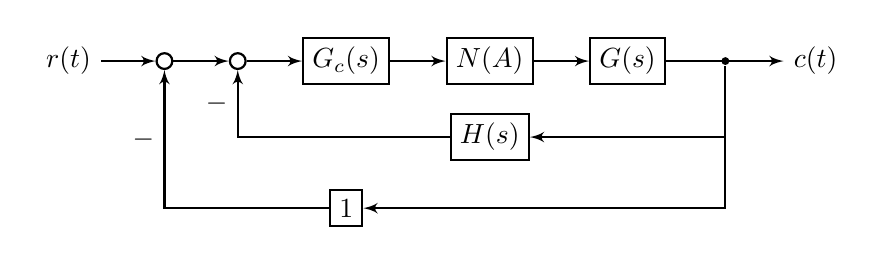
\begin{tikzpicture}[node distance=3em,auto,>=latex', thick]
%\path[use as bounding box] (-1,0) rectangle (10,-2); 
\tikzstyle{block} = [draw,rectangle,thick,minimum height=1em,minimum width=1em]
\tikzstyle{sum} = [draw,circle,inner sep=0mm,minimum size=2mm]
\tikzstyle{branch} = [circle,fill,inner sep=0pt,minimum size=1mm]
\tikzstyle{connector} = [->,thick]

\def\r{\node(r){$r(t)$};}
\def\b(#1){\node[branch](b#1){};}
\def\p(#1){\node[sum](p#1){};}
\def\gc{\node[block](gc){$G_c(s)$};}
\def\na{\node[block](na){$N(A)$};}
\def\gp{\node[block](gp){$G(s)$};}
\def\gh{\node[block](gh){$H(s)$};}
\def\g(#1){\node[block](g#1){$1$};}
\def\c{\node(c){$c(t)$};}

\matrix[ampersand replacement=\&, row sep=1em, column sep=2em]{
	\r  \&  \p(e)  \& \p(r) \& \gc \& \na \& \gp \& \b(c)  \& \c  \\
	\&         \&       \&      \& \gh  \\
	\&         \&       \& \g(h1)    \\
};
\draw [connector](r) -- (pe) ; 
\draw [connector](pe) -- (pr) ; 
\draw [connector](pr)-- (gc) ; 
\draw [connector](gc) -- (na) ; 
\draw [connector](na) -- (gp) ; 
\draw [connector](gp) -- (c) ; 
\draw [connector](bc) |- (gh) ; 
\draw [connector](bc) |- (gh1) ; 
\draw [connector](gh) -| node[near end , left]{$-$} (pr) ; 
\draw [connector](gh1) -| node[near end , left]{$-$} (pe) ; 
\end{tikzpicture} 

\onlyanswer
{
答:系统等效开环传递函数为:
\begin{align*}
G(s) &=\frac{1}{s(s+1)^2}
\end{align*}

计算Nyquist曲线与虚轴交点:
\begin{align*}
\omega_x &=1 \\
G(\omega_x) &= -\frac{1}{2}
\end{align*}
Nyquist曲线不包围负倒描述函数或与其相交:
\begin{align*}
-\frac{1}{N(A)} &< -\frac{1}{2} ,A\in(0,\infty)\\
-A-k&<-\frac{1}{2}\\
k &>\frac{1}{2}
\end{align*}
所以$k=1$时系统稳定无自振。
}

%\onlytest{\vskip 3em}
%\onlytest{\newpage}




\question(20分){已知控制系统结构图如下所示, 已知$r(t)=1,(t>0)$ 求解当$a=0$  时的 $Y(z)$ 与 $a\in(0,1]$ 时的 $Y(z)$ 。




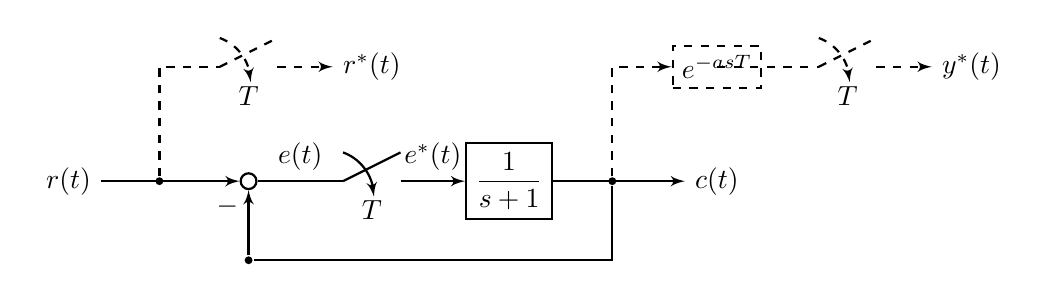
\begin{tikzpicture}[node distance=3em,auto,>=latex', thick]
%\path[use as bounding box] (-1,0) rectangle (10,-2); 
\tikzstyle{block} = [draw,rectangle,thick,minimum height=1em,minimum width=1em]
\tikzstyle{sum} = [draw,circle,inner sep=0mm,minimum size=2mm]
\tikzstyle{branch} = [circle,fill,inner sep=0pt,minimum size=1mm]
\tikzstyle{connector} = [->,thick]

\def\r{\node(r){$r(t)$};}
\def\rd{\node(rd){$r^*(t)$};}
\def\b(#1){\node[branch](b#1){};}
\def\p(#1){\node[sum](p#1){};}
\def\s(#1){\path[->] node[minimum size=2em] (s#1) {}; \draw (s#1.west)--(s#1.north east);\draw[->] (s#1.north west) arc (70:0:1.7em);\draw (s#1.south) node {$T$};}
\def\sd(#1){\path[->] node[minimum size=2em] (sd#1) {}; \draw[dashed] (sd#1.west)--(sd#1.north east);\draw[dashed,->] (sd#1.north west) arc (70:0:1.7em);\draw[dashed] (sd#1.south) node {$T$};}
\def\ga{\node[block](g1){$\dfrac{1}{s+1}$};}
\def\gb{\node[dashed,block](g2){$e^{-asT}$};}
\def\c{\node(c){$c(t)$};}
\def\cd{\node(cd){$y^*(t)$};}

\matrix[ampersand replacement=\&, row sep=1em, column sep=2em]{
	\&         \& \sd(r)  \& \rd   \&    \&         \&   \gb  \&  \sd(c)  \& \cd \\
\r  \& \b(r)   \& \p(e)   \& \s(e) \& \ga \&  \b(c)  \&  \c \\
	\&         \& \b(h) \\
};
\draw [connector](r) -- (pe) ; 
\draw [dashed](br)  |- (sdr) ; 
\draw [connector,dashed](sdr) -- (rd) ; 
\path[](pe) edge node[midway] {$e(t)$} (se) ; 
\draw [connector] (se) -- node[midway] {$e^*(t)$} (g1); 
\draw [connector] (g1) -- node[midway] {$   $} (c); 
\draw [dashed,connector](bc)  |- (g2) ; 
\draw [dashed](g2)  |- (sdc) ;
\draw [connector,dashed](sdc) -- (cd) ; 
\draw [](bc)  |- (bh) ; 
\draw [connector](bh) --  node[near end,left]{$-$} (pe) ; 
\end{tikzpicture} 

\comment{
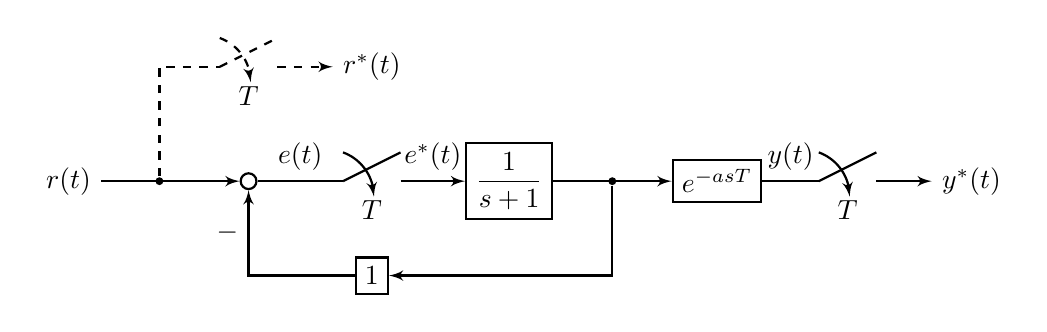
\begin{tikzpicture}[node distance=3em,auto,>=latex', thick]
%\path[use as bounding box] (-1,0) rectangle (10,-2); 
\tikzstyle{block} = [draw,rectangle,thick,minimum height=1em,minimum width=1em]
\tikzstyle{sum} = [draw,circle,inner sep=0mm,minimum size=2mm]
\tikzstyle{branch} = [circle,fill,inner sep=0pt,minimum size=1mm]
\tikzstyle{connector} = [->,thick]

\def\r{\node(r){$r(t)$};}
\def\rd{\node(rd){$r^*(t)$};}
\def\b(#1){\node[branch](b#1){};}
\def\p(#1){\node[sum](p#1){};}
\def\s(#1){\path[->] node[minimum size=2em] (s#1) {}; \draw (s#1.west)--(s#1.north east);\draw[->] (s#1.north west) arc (70:0:1.7em);\draw (s#1.south) node {$T$};}
\def\sd(#1){\path[->] node[minimum size=2em] (sd#1) {}; \draw[dashed] (sd#1.west)--(sd#1.north east);\draw[dashed,->] (sd#1.north west) arc (70:0:1.7em);\draw[dashed] (sd#1.south) node {$T$};}
\def\ga{\node[block](g1){$\dfrac{1}{s+1}$};}
\def\gb{\node[block](g2){$e^{-asT}$};}
\def\c{\node(c){$y(t)$};}
\def\cd{\node(cd){$y^*(t)$};}
\def\g(#1){\node[block](g#1){$1$};}

\matrix[ampersand replacement=\&, row sep=1em, column sep=2em]{
	\&         \& \sd(r)  \& \rd      \&  \&     \&          \&    \&  \\
	\r  \& \b(r)   \& \p(e)   \& \s(e) \& \ga \&  \b(c)  \&  \gb \&  \s(c) \& \cd \\
	\&         \& \           \& \g(h) \\
};
\draw [connector](r) -- (pe) ; 
\draw [dashed](br)  |- (sdr) ; 
\draw [connector,dashed](sdr) -- (rd) ; 
\path[](pe) edge node[midway] {$e(t)$} (se) ; 
\draw [connector] (se) -- node[midway] {$e^*(t)$} (g1); 
\draw [connector] (g1) -- node[midway] {$   $} (g2); 
%\draw [connector] (g2)-- (sc); 
\path[](g2) edge node[midway] {$y(t)$} (sc) ; 
\draw [connector] (sc)-- (cd); 
%\draw [dashed](bc)  |- (sdc) ; 
%\draw [connector,dashed](sdc) -- (cd) ; 
\draw [connector](bc)  |- (gh) ; 
\draw [connector](gh) -|  node[near end,left]{$-$} (pe) ; 
\end{tikzpicture} 

}%comment


\onlyanswer
{
	答:$a=0$ 时:
	
	\begin{align*}
	Y^*(s) &= \frac{[\frac{1}{s+1}]^*}{1+[\frac{1}{s+1}]^*}R^*(s) \\
	Y(z)  &= \frac{\frac{1}{1-e^{-T}z^{-1}}} {1+\frac{1}{1-e^{-T}z^{-1}}}\cdot\frac{1}{1-z^{-1}} \\
	&= \frac{1}{(2-e^{-T}z^{-1})(1-z^{-1})} 
	\end{align*}
	
	
	
	$a\in(0,1]$时:
	
	
	\begin{align*}
	Y^*(s) &= \left[\frac{e^{-aTs}}{s+1}\right]^*\frac{R^*_T(s)}{1+[\frac{1}{s+1}]^*} \\
	Y(z)  &={\cal Z}\left[\left[\frac{e^{-aTs}}{s+1}\right]^*\right]\cdot \frac{1}{1+\frac{1}{1-e^{-T}z^{-1}}}\cdot \frac{1}{1-z^{-1}} \\
	&=\frac{e^{aT}e^{-T}z^{-1}}{1-e^{-T}z^{-1}}\cdot \frac{1}{1+\frac{1}{1-e^{-T}z^{-1}}}\cdot \frac{1}{1-z^{-1}} \\
	&=\frac{e^{aT}e^{-T}z^{-1}}{(1-z^{-1})(2-e^{-T}z^{-1})}
	\end{align*}
	其中:
	\begin{align*}
	\frac{e^{-aTs}}{s+1} &= {\cal L}[e^{-(t-aT)}]\qquad (t\geq aT)  \\
	{\cal Z}[e^{-nT+aT} ] &= \sum_{n=1}^{\infty} e^{-nT+aT}z^{-n}\\
	&=\frac{e^{aT-T}z^-1}{1-e^{-T}z^-1}
	\end{align*}
}

}

\question(20分)已知控制系统结构图如下所示,已知 $G(s)=\frac{1}{s+1},G_c(s)=1$ 。 若 $G_r(s)=\frac{k_1 s+k_2}{s+1},r(t)=t,(t>0,k_2=1)$ , 如何选取 $k_1$ 使稳态误差为零?
若$G_r(s)=Ae^{-\theta s},r(t)=sin(t),(t>0)$ 如何选取 $A,\theta,(\theta\in(0,2\pi))$ 使系统稳态输出 $c(t)=sin(t)$ ?



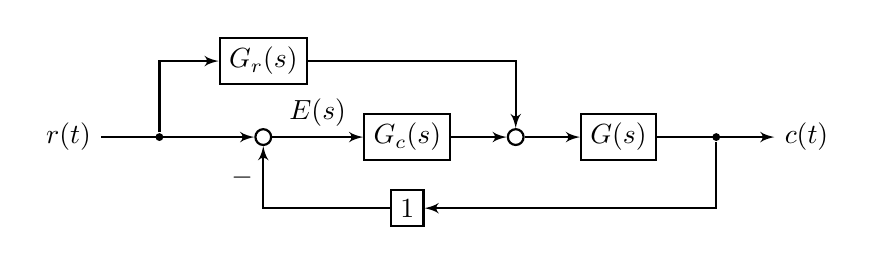
\begin{tikzpicture}[node distance=3em,auto,>=latex', thick]
%\path[use as bounding box] (-1,0) rectangle (10,-2); 
\tikzstyle{block} = [draw,rectangle,thick,minimum height=1em,minimum width=1em]
\tikzstyle{sum} = [draw,circle,inner sep=0mm,minimum size=2mm]
\tikzstyle{branch} = [circle,fill,inner sep=0pt,minimum size=1mm]
\tikzstyle{connector} = [->,thick]

\def\r{\node(r){$r(t)$};}
\def\b(#1){\node[branch](b#1){};}
\def\p(#1){\node[sum](p#1){};}
\def\gc{\node[block](gc){$G_c(s)$};}
\def\gr{\node[block](gr){$G_r(s)$};}
\def\gp{\node[block](gp){$G(s)$};}
\def\g(#1){\node[block](g#1){$1$};}
\def\c{\node(c){$c(t)$};}

\matrix[ampersand replacement=\&, row sep=1em, column sep=2em]{
	\&         \&   \gr  \\
	\r  \&   \b(r)  \& \p(e)  \& \gc \& \p(r) \& \gp \& \b(c)  \& \c  \\
	\&         \&         \& \g(h)    \\
};
\draw [connector](r) -- (pe) ; 
\draw [connector](br) |- (gr) ; 
\draw [connector](gr) -| (pr) ; 
\draw [connector](pe) -- node[midway]{$E(s)$} (gc) ; 
\draw [connector](gc) -- (pr) ; 
\draw [connector](pr) -- (gp) ; 
\draw [connector](gp) -- (c) ; 
\draw [connector](bc) |- (gh) ; 
\draw [connector](gh) -| node[near end , left]{$-$} (pe) ; 
\end{tikzpicture} 

\onlyanswer
{
	答:当 $G_r(s)=\frac{k_1 s+k_2}{s+1},r(t)=t,(t>0)$ 时,得:
	\begin{align*}
	\frac{E(s)}{R(s)} &= (1-\frac{k_1s+k_2}{s+1}\cdot\frac{1}{s+1})\frac{1}{1+\frac{1}{s+1}} \\
	&=\frac{(s+1)^2-(k_1s+k_2)}{(s+2)(s+1)} \\
	&=\frac{s^2+(2-k_1)s+(1-k_2)}{(s+2)(s+1)} \\
	&=\frac{s^2+(2-k_1)s}{(s+2)(s+1)} \\
	\end{align*}
	所以,当 $k_1=2,k_2=1$ 时,
	\begin{align*}
	E(s) &=\frac{s^2+(2-k_1)s+(1-k_2)}{(s+2)(s+1)}\cdot R(s) \\
	&=\frac{s^2}{(s+2)(s+1)}\cdot \frac{1}{s^2} \\
	&=\frac{1}{(s+2)(s+1)} \\
	e_{ss} &= \lim_{s\rightarrow 0} sE(s) \\
	&= 0
	\end{align*}
	
	当 $G_r(s)=Ae^{-\theta s},r(t)=sin(t),(t>0)$ 时:
	\begin{align*}
	G(j\omega) &=\frac{1}{j\omega+1} \\
	G_r(j\omega) &=Ae^{-j\theta\omega} \\
	\frac{C(j\omega)}{R(j\omega)} &= \frac{G(j\omega)+G_r(j\omega)G(j\omega)}{1+G(j\omega)} \\
	&=\frac{1+Ae^{-j\theta\omega}}{2+j\omega}
	\end{align*}
	
	稳态时,
	\begin{align*}
	\left.\frac{C(j\omega)}{R(j\omega)}\right|_{\omega=1} &=\left.\frac{1+Ae^{-j\theta\omega}}{2+j\omega}\right|_{\omega=1} \\
	&=\frac{1+Ae^{-j\theta}}{2+j} \\
	&=1 
	\end{align*}
	得:
	\begin{align*}
	A &=\sqrt{2} \\
	\theta &=2n\pi-\frac{\pi}{4}\\
	&=\frac{7\pi}{4}
	\end{align*}
}




\question(20分)单位负反馈系统开环传递函数:
$$G(s)=\frac{k}{s+1}\cdot e^{\frac{-3\pi}{4} s}$$
当 $k=1$ 时系统的稳定性如何?相角裕度是多少?若要使系统稳定,实数$k$的范围是什么?
\onlyanswer
{
	答:
	
	$|G(j\omega)|$是$\omega$的单调减函数,当$k=1,\omega=0$时,$|G(j\omega)|=1$,Nyquist曲线不包围(-1+0j),闭环系统稳定。此时$\angle G(j\omega)=0$,因此相角裕度$\gamma=180^\circ$。
	
	\begin{tikzpicture}[scale=1]
	\begin{axis}[
	grid=both,
	%axis x line=middle,axis y line= middle, 
	ylabel=$j$ ,xlabel=$  $ ,
	ymin=-1,ymax=0.6,xmin=-2,xmax=2,every axis plot post/.append style={mark=none}]
	\addplot[blue,thick,->]
	shell {
		octave -q --eval "s=i*(0:0.01:10)';g=1.0./(s+1).*exp(-3*pi/4*s);disp([real(g),imag(g)]);"
	};
	\end{axis}
	\end{tikzpicture}
	
	当$k>0,\omega=1$时, $\angle G(j\omega)=-\pi$,$|G(s)|=\frac{k}{\sqrt{2}}$,因此,当$0<k<\sqrt{2}$时,系统稳定。
	
	当$-1<k<0$时,Nyquist曲线不包围(-1+0j),系统稳定。
	当$k<-1$时,Nyquist曲线包围(-1+0j),系统不稳定。
	因此,当$-1<k<\sqrt{2}$时,闭环系统稳定。
	
	
}





\question(20分)单位负反馈控制系统开环传递函数,
$$G(s)=\frac{20}{s(s+1)(s+5)}$$
串联校正网络:
$$G_c(s)=k\cdot\frac{T_b s+1}{bT_b s+1}\cdot\frac{aT_a s+1}{T_a s+1}$$
求解参数 $b,a,T_a$ 使校正后系统截止频率不变,稳态性能不变,相角裕度提高约 $30^\circ$ 。(已知 $0<b<a,\frac{1}{T_b}\approx 0$)

\onlyanswer
{
	答:计算校正前截止频率:
	\begin{align*}
	|G(s)| &=1 \\
	\omega_c &=2 
	\end{align*}
	计算超前校正网络参数:
	\begin{align*}
	\sin 30^{\circ} &= \frac{a-1}{a+1}\\
	a &= 3 \\
	\frac{1}{\sqrt{a}T_a} &= \omega_c \\
	T_a &= \frac{1}{2\sqrt{3}} \\
	\end{align*}
	由系统稳态性能不变得:$k=1$ 。由截止频率保持不变,得:
	\begin{align*}
	\frac{1}{b}\cdot aT_a\omega_c &= 1 \\
	b &= \sqrt{3}
	\end{align*}
}



\comment{

\question(20分)已知控制系统结构图如下所示,求 $E_1(s),E_2(s)$


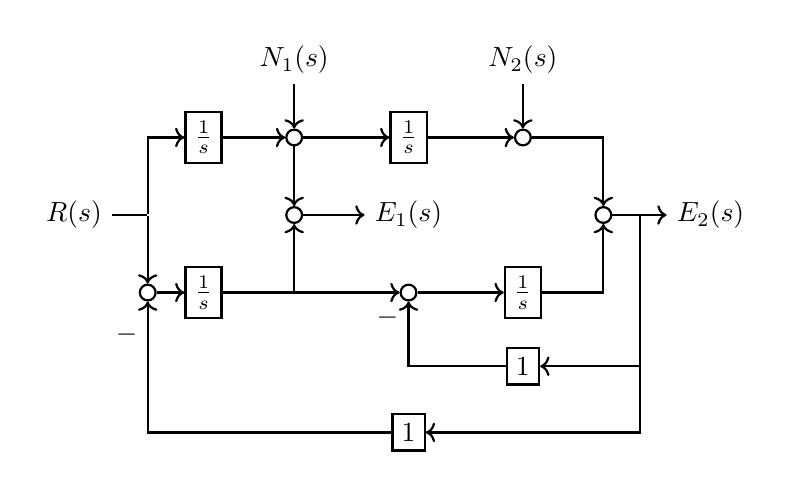
\begin{tikzpicture}[scale=1, thick] 
\tikzstyle{block} = [draw,rectangle,thick,minimum height=1em,minimum width=1em]
\tikzstyle{sum} = [draw,circle,inner sep=0mm,minimum size=2mm]
\tikzstyle{branch} = [inner sep=0pt,minimum size=0pt]
\tikzstyle{connector} = [->,thick]
\matrix[ampersand replacement=\&, row sep=1em, column sep=1em]{
\&  \&  \& \node(n1){$N_1(s)$};\&\&\node(n2){$N_2(s)$}; \\

\&  \&  \node[block](g1){$\frac{1}{s}$}; \& \node[sum](p1) {}; \& \node[block] (g2){$\frac{1}{s}$}; \& \node[sum](p2) {};  \\

\node[] (r) {$R(s)$}; \& 
\node[branch] (b1) {} ; \&
\&
\node[sum](p3) {}; \&
\node[] (e1) {$E_1(s)$} ; \&
\&
\node[sum](p4) {};\&
\node[branch] (b2) {} ;  \&
\node[] (e2) {$E_2(s)$} ; 
\\

\& \node[sum](p5) {}; \&  \node[block](g3){$\frac{1}{s}$}; \&  \&
\node[sum](p6) {}; \& \node[block](g4){$\frac{1}{s}$};   \\
\& \& \& \& \& \node[block](h1){$1$}; \\
\& \& \& \& \node[block](h2){$1$}; \\
};
\draw [connector] (n1) -- (p1);
\draw [connector] (n2) -- (p2);
\draw [thick] (r) -- (b1);
\draw [connector] (b1) |- (g1);
\draw [connector] (b1) -- (p5);
\draw [connector] (p5) -- (g3);
\draw [connector] (g1) -- (p1);
\draw [connector] (p1) -- (g2);\draw [connector] (p1) -- (p3);
\draw [connector] (g3) -- (p6);
\draw [connector] (p6) -- (g4);
\draw [connector] (g3) -| (p3);
\draw [connector] (p3) -- (e1);
\draw [connector] (g2) -- (p2);
\draw [connector] (p2) -| (p4);
\draw [connector] (g4) -| (p4);
\draw [connector] (p4) -- (e2);
\draw [connector] (b2) |- (h1);
\draw [connector] (b2) |- (h2);
\draw [connector] (h1) -|  node[very near end,left] {$-$} (p6);
\draw [connector] (h2) -|  node[very near end,left] {$-$} (p5);
\end{tikzpicture} 



\onlyanswer
{


}


\question(20分)已知单位负反馈系统开环传递函数:
$$G(s)=\frac{C(s)}{R(s)}=\frac{k}{s(s+a)}$$
若 $c(0)=1,c'(0)=1,r(t)=1+t$ 求系统稳态误差。

\question(20分)绘制系统根轨迹:
$$G(s)=\frac{K^*(s^2+a)}{s^2+b}$$


\question(20分)已知单位负反馈系统开环传递函数:
$$G(s)=\frac{\sqrt{2}}{s+1}\cdot e^{-\frac{3\pi}{4}s}$$
分析系统稳定性。

\question(20分)分析系统稳定性:
$$G(s)=\frac{K}{s+1}\cdot e^{-Ts}$$



\question(20分)已知控制系统模型如下:
\begin{align*}
\dot{y}(t) & =v(t) \\
\dot{v}(t) & =u(t) \\
u(t) &=e(t)-k_1 v(t)+k_2 \dot{r}(t)\\
e(t) &=r(t)- y(t)
\end{align*}
绘制系统结构图,推导传递函数$G(s)=\frac{Y(s)}{R(s)}$,当参考输入 $r(t)=t,(t>0)$ ,且 $\lim_{t\rightarrow\infty}e(t)=0$ 时, $k_1,k_2$可取何值。

\question(20分)已知系统结构图如下:

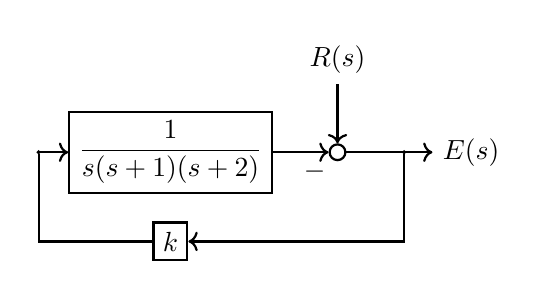
\begin{tikzpicture}[scale=1, thick] 
\tikzstyle{block} = [draw,rectangle,thick,minimum height=1em,minimum width=1em]
\tikzstyle{sum} = [draw,circle,inner sep=0mm,minimum size=2mm]
\tikzstyle{branch} = [draw,circle,fill,inner sep=0pt,minimum size=0.5pt]
\tikzstyle{connector} = [->,thick]
\matrix[ampersand replacement=\&, row sep=1em, column sep=1em]{
\& \&  \node(r){$R(s)$};\\

\node[branch](bc){};\& \node[block](g){$\dfrac{1}{s(s+1)(s+2)}$}; \& \node[sum](pe) {}; \& \node[branch] (be) {} ; \& \node(e){$E(s)$}; \\

 \&\node[block](gc){$k$};\\
};

\draw [connector] (r) -- (pe);
\draw [connector] (bc) --   (g);
\draw [connector] (g) -- node[near end,below] {$-$}(pe);
\draw [connector] (pe) -- (e);
\draw [connector] (be) |- (gc);
\draw [thick] (gc) -| (bc);
\end{tikzpicture} 

分析$k>0$时系统的稳定性,并求解当$R(s)=1,(t>0)$时信号$E(s)$的稳态值。

\question(20分)已知系统结构图如下:

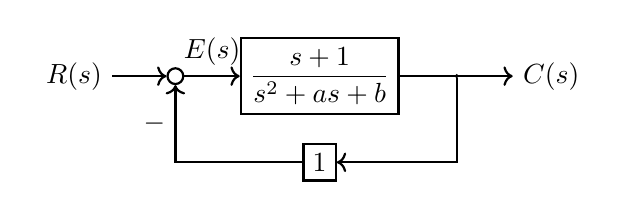
\begin{tikzpicture}[scale=1, thick] 
\tikzstyle{block} = [draw,rectangle,thick,minimum height=1em,minimum width=1em]
\tikzstyle{sum} = [draw,circle,inner sep=0mm,minimum size=2mm]
\tikzstyle{branch} = [draw,circle,fill,inner sep=0pt,minimum size=0.5pt]
\tikzstyle{connector} = [->,thick]
\matrix[ampersand replacement=\&, row sep=1em, column sep=2em]{
\node(r){$R(s)$};\&\node[sum](pe){};\& \node[block](g){$\dfrac{s+1}{s^2+as+b}$};\&\node[branch](bc) {} ; \& \node(c){$C(s)$}; \\

\& \& \node[block](gc){$1$};\\
};

\draw [connector] (r) -- (pe);
\draw [connector] (pe) -- node[midway,above] {$E(s)$} (g);
\draw [connector] (g) -- (c);
\draw [connector] (bc) |- (gc);
\draw [connector] (gc) -| node[near end,left] {$-$} (pe);
\end{tikzpicture} 

分析$a=1,b=1,R(s)=\frac{1}{s}$时系统的稳态误差。是否可通过改变$a,b$的值使得$R(s)=1/(s^2+1)$时稳态误差等于零。




\question(20分)已知控制系统结构图如下所示,已知 $r(t)=1,(t>0)$ 求 $y^*(t)$

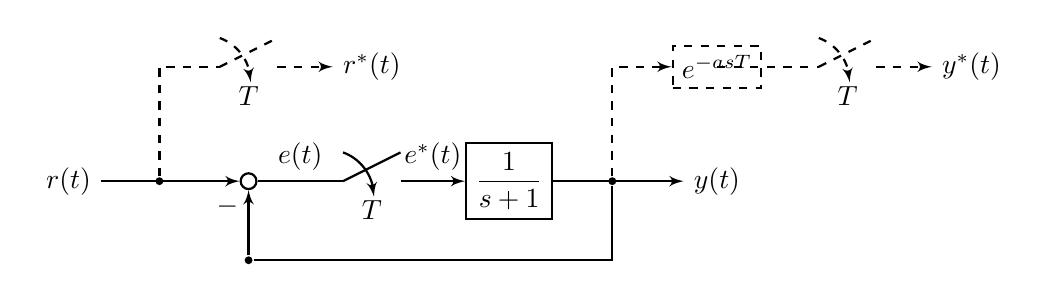
\begin{tikzpicture}[node distance=3em,auto,>=latex', thick]
%\path[use as bounding box] (-1,0) rectangle (10,-2); 
\tikzstyle{block} = [draw,rectangle,thick,minimum height=1em,minimum width=1em]
\tikzstyle{sum} = [draw,circle,inner sep=0mm,minimum size=2mm]
\tikzstyle{branch} = [circle,fill,inner sep=0pt,minimum size=1mm]
\tikzstyle{connector} = [->,thick]

\def\r{\node(r){$r(t)$};}
\def\rd{\node(rd){$r^*(t)$};}
\def\b(#1){\node[branch](b#1){};}
\def\p(#1){\node[sum](p#1){};}
\def\s(#1){\path[->] node[minimum size=2em] (s#1) {}; \draw (s#1.west)--(s#1.north east);\draw[->] (s#1.north west) arc (70:0:1.7em);\draw (s#1.south) node {$T$};}
\def\sd(#1){\path[->] node[minimum size=2em] (sd#1) {}; \draw[dashed] (sd#1.west)--(sd#1.north east);\draw[dashed,->] (sd#1.north west) arc (70:0:1.7em);\draw[dashed] (sd#1.south) node {$T$};}
\def\ga{\node[block](g1){$\dfrac{1}{s+1}$};}
\def\gb{\node[dashed,block](g2){$e^{-asT}$};}
\def\c{\node(c){$y(t)$};}
\def\cd{\node(cd){$y^*(t)$};}

\matrix[ampersand replacement=\&, row sep=1em, column sep=2em]{
	\&         \& \sd(r)  \& \rd   \&    \&         \&   \gb  \&  \sd(c)  \& \cd \\
\r  \& \b(r)   \& \p(e)   \& \s(e) \& \ga \&  \b(c)  \&  \c \\
	\&         \& \b(h) \\
};
\draw [connector](r) -- (pe) ; 
\draw [dashed](br)  |- (sdr) ; 
\draw [connector,dashed](sdr) -- (rd) ; 
\path[](pe) edge node[midway] {$e(t)$} (se) ; 
\draw [connector] (se) -- node[midway] {$e^*(t)$} (g1); 
\draw [connector] (g1) -- node[midway] {$   $} (c); 
\draw [dashed,connector](bc)  |- (g2) ; 
\draw [dashed](g2)  |- (sdc) ;
\draw [connector,dashed](sdc) -- (cd) ; 
\draw [](bc)  |- (bh) ; 
\draw [connector](bh) --  node[near end,left]{$-$} (pe) ; 
\end{tikzpicture} 



\question(20分)已知控制系统结构图如下所示, 已知 $r(t)=1,(t>0)$ 。 当 $T_y=T,a=0$  时求解 $Y(z)$ ;当 $T_y=\frac{T}{2},a=1$ 时求解 $Y(z)$。

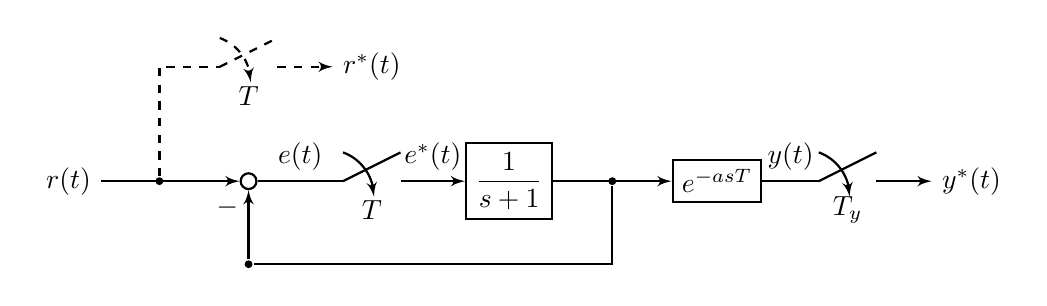
\begin{tikzpicture}[node distance=3em,auto,>=latex', thick]
%\path[use as bounding box] (-1,0) rectangle (10,-2); 
\tikzstyle{block} = [draw,rectangle,thick,minimum height=1em,minimum width=1em]
\tikzstyle{sum} = [draw,circle,inner sep=0mm,minimum size=2mm]
\tikzstyle{branch} = [circle,fill,inner sep=0pt,minimum size=1mm]
\tikzstyle{connector} = [->,thick]

\def\r{\node(r){$r(t)$};}
\def\rd{\node(rd){$r^*(t)$};}
\def\b(#1){\node[branch](b#1){};}
\def\p(#1){\node[sum](p#1){};}
\def\s(#1){\path[->] node[minimum size=2em] (s#1) {}; \draw (s#1.west)--(s#1.north east);\draw[->] (s#1.north west) arc (70:0:1.7em);\draw (s#1.south) node {$T$};}
\def\sz(#1){\path[->] node[minimum size=2em] (sz#1) {}; \draw (sz#1.west)--(sz#1.north east);\draw[->] (sz#1.north west) arc (70:0:1.7em);\draw (sz#1.south) node {$T_y$};}
\def\sd(#1){\path[->] node[minimum size=2em] (sd#1) {}; \draw[dashed] (sd#1.west)--(sd#1.north east);\draw[dashed,->] (sd#1.north west) arc (70:0:1.7em);\draw[dashed] (sd#1.south) node {$T$};}
\def\ga{\node[block](g1){$\dfrac{1}{s+1}$};}
\def\gb{\node[block](g2){$e^{-asT}$};}
\def\c{\node(c){$y(t)$};}
\def\cd{\node(cd){$y^*(t)$};}

\matrix[ampersand replacement=\&, row sep=1em, column sep=2em]{
	\&         \& \sd(r)  \& \rd      \&  \&     \&          \&    \&  \\
	\r  \& \b(r)   \& \p(e)   \& \s(e) \& \ga \&  \b(c)  \&  \gb \&  \sz(c) \& \cd \\
	\&         \& \b(h) \\
};
\draw [connector](r) -- (pe) ; 
\draw [dashed](br)  |- (sdr) ; 
\draw [connector,dashed](sdr) -- (rd) ; 
\path[](pe) edge node[midway] {$e(t)$} (se) ; 
\draw [connector] (se) -- node[midway] {$e^*(t)$} (g1); 
\draw [connector] (g1) -- node[midway] {$   $} (g2); 
\path[](g2) edge node[midway] {$y(t)$} (szc) ; 
\draw [connector] (szc)-- (cd); 
\draw [](bc)  |- (bh) ; 
\draw [connector](bh) --  node[near end,left]{$-$} (pe) ; 
\end{tikzpicture} 

\onlyanswer
{
	答:$a=0,T_y=T$ 时:
	
	\begin{align*}
	Y^*(s) &= \frac{[\frac{1}{s+1}]^*}{1+[\frac{1}{s+1}]^*}R^*(s) \\
	Y(z)  &= \frac{\frac{1}{1-e^{-T}z^{-1}}}{1+\frac{1}{1-e^{-T}z^{-1}}}\frac{1}{1-z^{-1}} \\
	&= \frac{1}{(2-e^{-T}z^{-1})(1-z^{-1})} 
	\end{align*}
	
	
	
	$T_y=\frac{T}{2},a=0$时,可采用修正 $Z$ 变换方法计算。
	
	
	\begin{align*}
	Y^*(s) &= \left[\frac{1}{s+1}\cdot\frac{R^*_T(s)}{1+[\frac{1}{s+1}]^*_T}\right]^*_{\frac{T}{2}} \\
	Y(z)  &={\cal Z}_{\frac{T}{2}}\left[\left[\frac{1}{s+1}\right]^*_{\frac{T}{2}}\right]{\cal Z}_{\frac{T}{2}}\left[\frac{R^*_T(s)}{1+[\frac{1}{s+1}]^*_T}\right] \\
	&=\frac{1}{1-e^{-T/2}z^{-1}}
	\cdot \frac{\frac{1}{1-z^{-2}}}{1+\frac{1}{1-e^{-T}z^{-2}}} \\
	&= \frac{1-e^{-T}z^{-2}}{(1-e^{-T/2}z^{-1})(2-e^{-T}z^{-2})(1-z^{-2})} 
	\end{align*}
	
}


\question(20分)已知控制系统结构图如下所示, 已知$r(t)=1,(t>0)$ 求解当$a=0$  时的 $Y(z)$ 。当 $a=\frac{1}{2}$ 时给出$y(nT)$的求解方法。

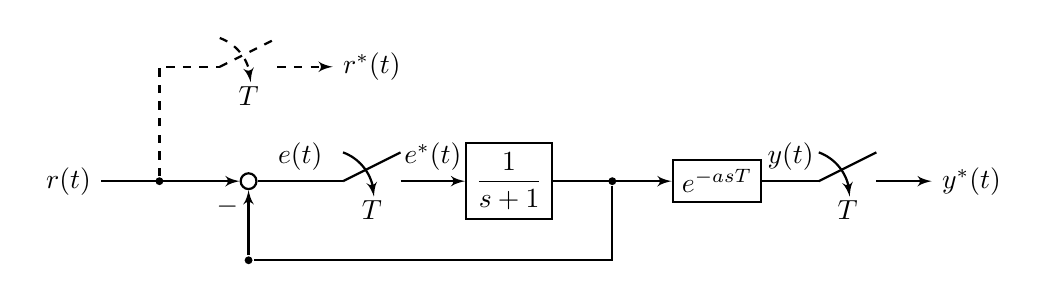
\begin{tikzpicture}[node distance=3em,auto,>=latex', thick]
%\path[use as bounding box] (-1,0) rectangle (10,-2); 
\tikzstyle{block} = [draw,rectangle,thick,minimum height=1em,minimum width=1em]
\tikzstyle{sum} = [draw,circle,inner sep=0mm,minimum size=2mm]
\tikzstyle{branch} = [circle,fill,inner sep=0pt,minimum size=1mm]
\tikzstyle{connector} = [->,thick]

\def\r{\node(r){$r(t)$};}
\def\rd{\node(rd){$r^*(t)$};}
\def\b(#1){\node[branch](b#1){};}
\def\p(#1){\node[sum](p#1){};}
\def\s(#1){\path[->] node[minimum size=2em] (s#1) {}; \draw (s#1.west)--(s#1.north east);\draw[->] (s#1.north west) arc (70:0:1.7em);\draw (s#1.south) node {$T$};}
\def\sd(#1){\path[->] node[minimum size=2em] (sd#1) {}; \draw[dashed] (sd#1.west)--(sd#1.north east);\draw[dashed,->] (sd#1.north west) arc (70:0:1.7em);\draw[dashed] (sd#1.south) node {$T$};}
\def\ga{\node[block](g1){$\dfrac{1}{s+1}$};}
\def\gb{\node[block](g2){$e^{-asT}$};}
\def\c{\node(c){$y(t)$};}
\def\cd{\node(cd){$y^*(t)$};}

\matrix[ampersand replacement=\&, row sep=1em, column sep=2em]{
	\&         \& \sd(r)  \& \rd      \&  \&     \&          \&    \&  \\
	\r  \& \b(r)   \& \p(e)   \& \s(e) \& \ga \&  \b(c)  \&  \gb \&  \s(c) \& \cd \\
	\&         \& \b(h) \\
};
\draw [connector](r) -- (pe) ; 
\draw [dashed](br)  |- (sdr) ; 
\draw [connector,dashed](sdr) -- (rd) ; 
\path[](pe) edge node[midway] {$e(t)$} (se) ; 
\draw [connector] (se) -- node[midway] {$e^*(t)$} (g1); 
\draw [connector] (g1) -- node[midway] {$   $} (g2); 
%\draw [connector] (g2)-- (sc); 
\path[](g2) edge node[midway] {$y(t)$} (sc) ; 
\draw [connector] (sc)-- (cd); 
%\draw [dashed](bc)  |- (sdc) ; 
%\draw [connector,dashed](sdc) -- (cd) ; 
\draw [](bc)  |- (bh) ; 
\draw [connector](bh) --  node[near end,left]{$-$} (pe) ; 
\end{tikzpicture} 

\onlyanswer
{
	答:$a=0$ 时:
	
	\begin{align*}
	Y^*(s) &= \frac{[\frac{1}{s+1}]^*}{1+[\frac{1}{s+1}]^*}R^*(s) \\
	Y(z)  &= \frac{\frac{1}{1-e^{-T}z^{-1}}}{1+\frac{1}{1-e^{-T}z^{-1}}}\frac{1}{1-z^{-1}} \\
	&= \frac{1}{(2-e^{-T}z^{-1})(1-z^{-1})} 
	\end{align*}
	
	
	
	$a=\frac{1}{2}$时,可采用修正 $Z$ 变换求得以 $\frac{T}{2}$ 采样得到的 $y(\frac{nT}{2})$ 后再令 $n$ 为奇数即可。
	
	
	\begin{align*}
	Y^*_{\frac{T}{2}}(s) &= \left[\frac{1}{s+1}\right]^*_{\frac{T}{2}}\left[\frac{R^*_T(s)}{1+[\frac{1}{s+1}]^*_T}\right]^*_{\frac{T}{2}} \\
	Y_{\frac{T}{2}}(z)  &=\frac{1}{1-e^{-T/2}z^{-1}} \frac{\frac{1}{1-z^{-2}}}{1+\frac{1}{1-e^{-T}z^{-2}}} \\
	&= \frac{1-e^{-T}z^{-2}}{(1-e^{-T/2}z^{-1})(2-e^{-T}z^{-2})(1-z^{-2})} 
	\end{align*}
	
}


\question(20分){已知控制系统结构图如下所示, 已知$r(t)=1,(t>0)$ 求解当$a=0$ 与 $a=\frac{1}{2}$ 时的 $Y(z)$ 。

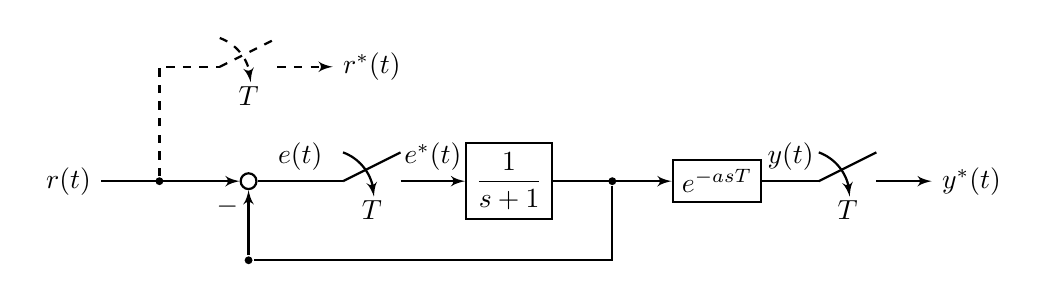
\begin{tikzpicture}[node distance=3em,auto,>=latex', thick]
%\path[use as bounding box] (-1,0) rectangle (10,-2); 
\tikzstyle{block} = [draw,rectangle,thick,minimum height=1em,minimum width=1em]
\tikzstyle{sum} = [draw,circle,inner sep=0mm,minimum size=2mm]
\tikzstyle{branch} = [circle,fill,inner sep=0pt,minimum size=1mm]
\tikzstyle{connector} = [->,thick]

\def\r{\node(r){$r(t)$};}
\def\rd{\node(rd){$r^*(t)$};}
\def\b(#1){\node[branch](b#1){};}
\def\p(#1){\node[sum](p#1){};}
\def\s(#1){\path[->] node[minimum size=2em] (s#1) {}; \draw (s#1.west)--(s#1.north east);\draw[->] (s#1.north west) arc (70:0:1.7em);\draw (s#1.south) node {$T$};}
\def\sd(#1){\path[->] node[minimum size=2em] (sd#1) {}; \draw[dashed] (sd#1.west)--(sd#1.north east);\draw[dashed,->] (sd#1.north west) arc (70:0:1.7em);\draw[dashed] (sd#1.south) node {$T$};}
\def\ga{\node[block](g1){$\dfrac{1}{s+1}$};}
\def\gb{\node[block](g2){$e^{-asT}$};}
\def\c{\node(c){$y(t)$};}
\def\cd{\node(cd){$y^*(t)$};}

\matrix[ampersand replacement=\&, row sep=1em, column sep=2em]{
	\&         \& \sd(r)  \& \rd      \&  \&     \&          \&    \&  \\
	\r  \& \b(r)   \& \p(e)   \& \s(e) \& \ga \&  \b(c)  \&  \gb \&  \s(c) \& \cd \\
	\&         \& \b(h) \\
};
\draw [connector](r) -- (pe) ; 
\draw [dashed](br)  |- (sdr) ; 
\draw [connector,dashed](sdr) -- (rd) ; 
\path[](pe) edge node[midway] {$e(t)$} (se) ; 
\draw [connector] (se) -- node[midway] {$e^*(t)$} (g1); 
\draw [connector] (g1) -- node[midway] {$   $} (g2); 
%\draw [connector] (g2)-- (sc); 
\path[](g2) edge node[midway] {$y(t)$} (sc) ; 
\draw [connector] (sc)-- (cd); 
%\draw [dashed](bc)  |- (sdc) ; 
%\draw [connector,dashed](sdc) -- (cd) ; 
\draw [](bc)  |- (bh) ; 
\draw [connector](bh) --  node[near end,left]{$-$} (pe) ; 
\end{tikzpicture} 

\onlyanswer
{
}

}



%\onlytest{\vskip 3em}

%\onlytest{\newpage}


\question(20分)已知控制系统结构图如下所示,

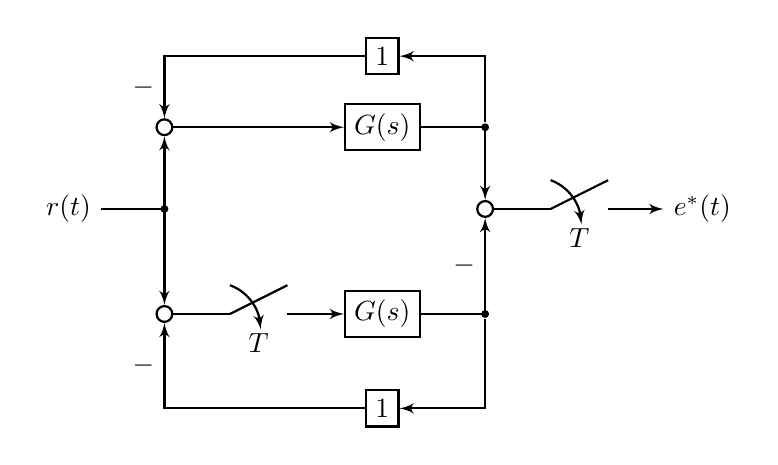
\begin{tikzpicture}[node distance=3em,auto,>=latex', thick]
%\path[use as bounding box] (-1,0) rectangle (10,-2); 
\tikzstyle{block} = [draw,rectangle,thick,minimum height=1em,minimum width=1em]
\tikzstyle{sum} = [draw,circle,inner sep=0mm,minimum size=2mm]
\tikzstyle{branch} = [circle,fill,inner sep=0pt,minimum size=1mm]
\tikzstyle{connector} = [->,thick]

\def\r{\node(r){$r(t)$};}
\def\rd{\node(rd){$r^*(t)$};}
\def\b(#1){\node[branch](b#1){};}
\def\p(#1){\node[sum](p#1){};}
\def\s(#1){\path[->] node[minimum size=2em] (s#1) {}; \draw (s#1.west)--(s#1.north east);\draw[->] (s#1.north west) arc (70:0:1.7em);\draw (s#1.south) node {$T$};}
\def\sd(#1){\path[->] node[minimum size=2em] (sd#1) {}; \draw[dashed] (sd#1.west)--(sd#1.north east);\draw[dashed,->] (sd#1.north west) arc (70:0:1.7em);\draw[dashed] (sd#1.south) node {$T$};}
\def\gc{\node[block](gc){$G(s)$};}
\def\gd{\node[block](gd){$G(s)$};}
\def\g(#1){\node[block](g#1){$1$};}
\def\ed{\node(ed){$e^*(t)$};}

\matrix[ampersand replacement=\&, row sep=1em, column sep=2em]{
	\&         \&   \& \g(ch)    \\
	\&  \p(ce) \&   \& \gc  \& \b(c)    \\  
\r  \&   \b(r)   \&   \&        \& \p(e)   \&  \s(e)  \& \ed  \\
	\&  \p(de) \& \s(de)  \& \gd  \& \b(d)    \\  
	\&         \&   \& \g(dh)    \\
};
\draw [connector](r) -| (pce) ; 
\draw [connector](r) -| (pde) ; 
\draw [connector](pce) -- (gc) ; 
\draw [connector](gc) -| (pe) ; 
\draw [connector](bc) |- (gch) ; 
\draw [connector](gch) -| node[near end , left]{$-$} (pce) ; 
\draw [](pde) -- (sde) ;
\draw [connector](sde) -- (gd) ;  
\draw [connector](gd) -| node[near end , left ]{$-$} (pe) ; 
\draw [connector](bd) |- (gdh) ; 
\draw [connector](gdh) -| node[near end , left ]{$-$} (pde) ; 
\draw [](pe)  -- (se) ; 
\draw [connector](se) -- (ed) ; 
\end{tikzpicture} 

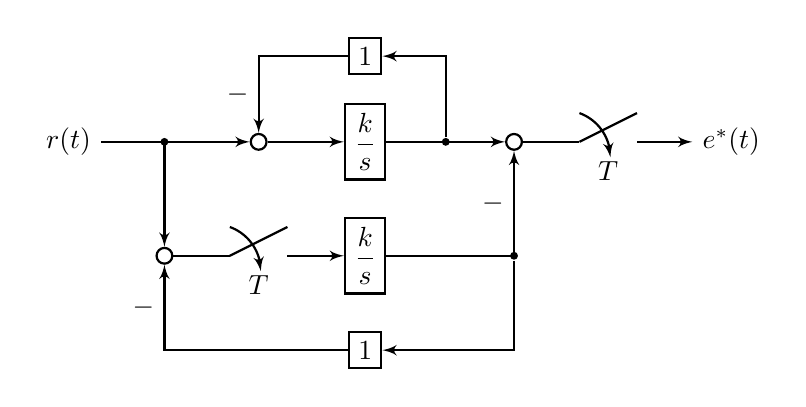
\begin{tikzpicture}[node distance=3em,auto,>=latex', thick]
%\path[use as bounding box] (-1,0) rectangle (10,-2); 
\tikzstyle{block} = [draw,rectangle,thick,minimum height=1em,minimum width=1em]
\tikzstyle{sum} = [draw,circle,inner sep=0mm,minimum size=2mm]
\tikzstyle{branch} = [circle,fill,inner sep=0pt,minimum size=1mm]
\tikzstyle{connector} = [->,thick]

\def\r{\node(r){$r(t)$};}
\def\rd{\node(rd){$r^*(t)$};}
\def\b(#1){\node[branch](b#1){};}
\def\p(#1){\node[sum](p#1){};}
\def\s(#1){\path[->] node[minimum size=2em] (s#1) {}; \draw (s#1.west)--(s#1.north east);\draw[->] (s#1.north west) arc (70:0:1.7em);\draw (s#1.south) node {$T$};}
\def\sd(#1){\path[->] node[minimum size=2em] (sd#1) {}; \draw[dashed] (sd#1.west)--(sd#1.north east);\draw[dashed,->] (sd#1.north west) arc (70:0:1.7em);\draw[dashed] (sd#1.south) node {$T$};}
\def\gc{\node[block](gc){$\dfrac{k}{s}$};}
\def\gd{\node[block](gd){$\dfrac{k}{s}$};}
\def\g(#1){\node[block](g#1){$1$};}
\def\ed{\node(ed){$e^*(t)$};}

\matrix[ampersand replacement=\&, row sep=1em, column sep=2em]{
	\&         \&   \& \g(ch)    \\
\r  \&   \b(r)  \& \p(ce)  \& \gc  \& \b(c)  \& \p(e)   \&  \s(e)  \& \ed  \\
	\&  \p(de) \& \s(de)  \& \gd  \& \& \b(d)    \\  
	\&         \&   \& \g(dh)    \\
};
\draw [connector](r) -- (pce) ; 
\draw [connector](r) -| (pde) ; 
\draw [connector](pce) -- (gc) ; 
\draw [connector](gc) -- (pe) ; 
\draw [connector](bc) |- (gch) ; 
\draw [connector](gch) -| node[near end , left]{$-$} (pce) ; 
\draw [](pde) -- (sde) ;
\draw [connector](sde) -- (gd) ;  
\draw [connector](gd) -| node[near end , left ]{$-$} (pe) ; 
\draw [connector](bd) |- (gdh) ; 
\draw [connector](gdh) -| node[near end , left ]{$-$} (pde) ; 
\draw [](pe)  -- (se) ; 
\draw [connector](se) -- (ed) ; 
\end{tikzpicture} 

计算$r(t)=1,(t>0)$时的 $e^*(t)$,并分析使系统稳定的 $k$ 取值范围。 
\onlyanswer
{
}


\question(20分)单位负反馈控制系统开环传递函数,
$$G(s)=\frac{20}{s(s+1)(s+5)}$$
设计串联校正网络:
$$G_c(s)=k\cdot\frac{T_b s+1}{s}\cdot\frac{aT_a s+1}{T_a s+1}$$
使系统截止频率保持不变,同时使相角裕度提高 $30^\circ$ 以上。



\question(20分)单位负反馈控制系统开环传递函数,
$$G(s)=\frac{20}{s(s+1)(s+5)}$$
设计串联校正网络:
$$G_c(s)=k\cdot\frac{T_b s+1}{bT_b s+1}\cdot\frac{aT_a s+1}{T_a s+1}$$
使系统截止频率保持不变,同时使相角裕度提高约 $60^\circ$ 。(已知 $0<b<1,\frac{1}{T_b}\approx 0$)


\question(20分)已知控制系统结构图如下所示,已知 $G(s)=\frac{1}{s(s+1)},G_c(s)=k_1,G_r(s)=\frac{k_2 s+k_3}{s+1},r(t)=t^2,(t>0)$ 求 $k2,k3$ 使稳态误差为零。
若$G(s)=\frac{1}{(s+1)},G_c(s)=1,G_r(s)=\sqrt{2}e^{-\frac{7\pi}{4}s},r(t)=sin(t),(t>0)$ 求 $Y(j\omega),E(j\omega)$。


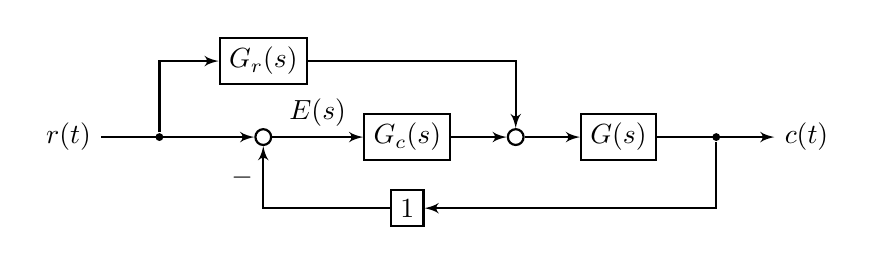
\begin{tikzpicture}[node distance=3em,auto,>=latex', thick]
%\path[use as bounding box] (-1,0) rectangle (10,-2); 
\tikzstyle{block} = [draw,rectangle,thick,minimum height=1em,minimum width=1em]
\tikzstyle{sum} = [draw,circle,inner sep=0mm,minimum size=2mm]
\tikzstyle{branch} = [circle,fill,inner sep=0pt,minimum size=1mm]
\tikzstyle{connector} = [->,thick]

\def\r{\node(r){$r(t)$};}
\def\b(#1){\node[branch](b#1){};}
\def\p(#1){\node[sum](p#1){};}
\def\gc{\node[block](gc){$G_c(s)$};}
\def\gr{\node[block](gr){$G_r(s)$};}
\def\gp{\node[block](gp){$G(s)$};}
\def\g(#1){\node[block](g#1){$1$};}
\def\c{\node(c){$c(t)$};}

\matrix[ampersand replacement=\&, row sep=1em, column sep=2em]{
	\&         \&   \gr  \\
	\r  \&   \b(r)  \& \p(e)  \& \gc \& \p(r) \& \gp \& \b(c)  \& \c  \\
	\&         \&         \& \g(h)    \\
};
\draw [connector](r) -- (pe) ; 
\draw [connector](br) |- (gr) ; 
\draw [connector](gr) -| (pr) ; 
\draw [connector](pe) -- node[midway]{$E(s)$} (gc) ; 
\draw [connector](gc) -- (pr) ; 
\draw [connector](pr) -- (gp) ; 
\draw [connector](gp) -- (c) ; 
\draw [connector](bc) |- (gh) ; 
\draw [connector](gh) -| node[near end , left]{$-$} (pe) ; 
\end{tikzpicture} 



\question(20分)已知控制系统结构图如下所示,已知 $G(s)=\frac{1}{s+1},G_c(s)=1$ , 当 $G_r(s)=\frac{k_1 s+k_2}{s+1},r(t)=t,(t>0)$ 时, 求 $k_1,k_2$ 使稳态误差为零。
若$G_r(s)=Ae^{-\theta s},r(t)=sin(t),(t>0)$ 求 $A,\theta,(\theta\in(0,2\pi))$ 使系统稳态误差为零。


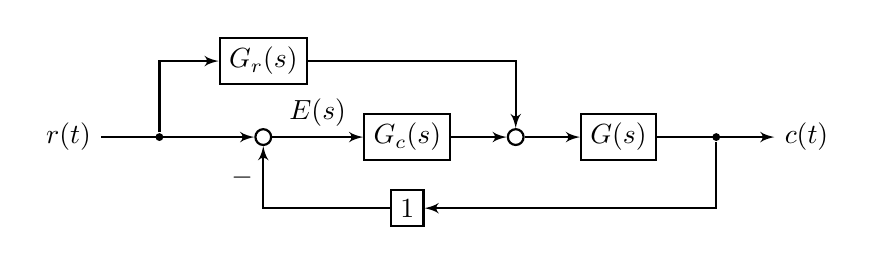
\begin{tikzpicture}[node distance=3em,auto,>=latex', thick]
%\path[use as bounding box] (-1,0) rectangle (10,-2); 
\tikzstyle{block} = [draw,rectangle,thick,minimum height=1em,minimum width=1em]
\tikzstyle{sum} = [draw,circle,inner sep=0mm,minimum size=2mm]
\tikzstyle{branch} = [circle,fill,inner sep=0pt,minimum size=1mm]
\tikzstyle{connector} = [->,thick]

\def\r{\node(r){$r(t)$};}
\def\b(#1){\node[branch](b#1){};}
\def\p(#1){\node[sum](p#1){};}
\def\gc{\node[block](gc){$G_c(s)$};}
\def\gr{\node[block](gr){$G_r(s)$};}
\def\gp{\node[block](gp){$G(s)$};}
\def\g(#1){\node[block](g#1){$1$};}
\def\c{\node(c){$c(t)$};}

\matrix[ampersand replacement=\&, row sep=1em, column sep=2em]{
	\&         \&   \gr  \\
	\r  \&   \b(r)  \& \p(e)  \& \gc \& \p(r) \& \gp \& \b(c)  \& \c  \\
	\&         \&         \& \g(h)    \\
};
\draw [connector](r) -- (pe) ; 
\draw [connector](br) |- (gr) ; 
\draw [connector](gr) -| (pr) ; 
\draw [connector](pe) -- node[midway]{$E(s)$} (gc) ; 
\draw [connector](gc) -- (pr) ; 
\draw [connector](pr) -- (gp) ; 
\draw [connector](gp) -- (c) ; 
\draw [connector](bc) |- (gh) ; 
\draw [connector](gh) -| node[near end , left]{$-$} (pe) ; 
\end{tikzpicture} 

\onlyanswer
{
	答:当 $G_r(s)=\frac{k_1 s+k_2}{s+1},r(t)=t,(t>0)$ 时,得:
	\begin{align*}
	\frac{E(s)}{R(s)} &= \frac{k_1s+k_2}{s+1}\cdot\frac{1}{s+1}\frac{1}{1+\frac{1}{s+1}} \\
	&=\frac{(s+1)^2-(k_1s+k_2)}{(s+2)(s+1)} \\
	&=\frac{s^2+(2-k_1)s+(1-k_2)}{(s+2)(s+1)} \\
	\end{align*}
	所以,当 $k_1=2,k_2=1$ 时,
	\begin{align*}
	E(s) &=\frac{s^2+(2-k_1)s+(1-k_2)}{(s+2)(s+1)}\cdot R(s) \\
	&=\frac{s^2}{(s+2)(s+1)}\cdot \frac{1}{s^2} \\
	&=\frac{1}{(s+2)(s+1)} \\
	e_{ss} &= \lim_{s\rightarrow 0} sE(s) \\
	&= 0
	\end{align*}
	
	当 $G_r(s)=Ae^{-\theta s},r(t)=sin(t),(t>0)$ 时:
	\begin{align*}
	G(j\omega) &=\frac{1}{j\omega+1} \\
	G_r(j\omega) &=Ae^{-j\theta\omega} \\
	\frac{E(j\omega)}{R(j\omega)} &= \frac{1-G_r(j\omega)}{1+G(j\omega)} \\
	&=\frac{1+j\omega-Ae^{-j\theta\omega}}{2+j\omega}
	\end{align*}
	
	稳态时,
	\begin{align*}
	\left.E(j\omega)\right|_{\omega=1} &=\left.\frac{1+j\omega-Ae^{-j\theta\omega}}{2+j\omega}\right|_{\omega=1} \\
	&=\frac{1+1j-Ae^{-j\theta}}{2+j} \\
	&=0 
	\end{align*}
	得:
	\begin{align*}
	A &=\sqrt{2} \\
	\theta &=2n\pi-\frac{\pi}{4}\\
	&=\frac{7\pi}{4}
	\end{align*}
	
}





\question(20分)已知控制系统结构图如下所示,已知 $N(A)=\frac{4}{\pi A}$ 分析系统稳定性,是否存在自振振荡?(若存在自激振荡需求出自振频率)



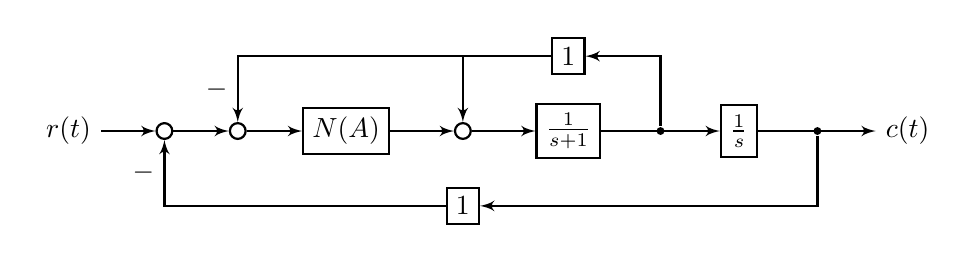
\begin{tikzpicture}[node distance=3em,auto,>=latex', thick]
%\path[use as bounding box] (-1,0) rectangle (10,-2); 
\tikzstyle{block} = [draw,rectangle,thick,minimum height=1em,minimum width=1em]
\tikzstyle{sum} = [draw,circle,inner sep=0mm,minimum size=2mm]
\tikzstyle{branch} = [circle,fill,inner sep=0pt,minimum size=1mm]
\tikzstyle{connector} = [->,thick]

\def\r{\node(r){$r(t)$};}
\def\b(#1){\node[branch](b#1){};}
\def\p(#1){\node[sum](p#1){};}
\def\na{\node[block](na){$N(A)$};} % y=sign(x)
\def\ga{\node[block](ga){$\frac{1}{s+1}$};}
\def\gb{\node[block](gb){$\frac{1}{s}$};}
\def\g(#1){\node[block](g#1){$1$};}
\def\c{\node(c){$c(t)$};}

\matrix[ampersand replacement=\&, row sep=1em, column sep=2em]{
	\&         \&       \&     \&       \&   \g(h1) \\
\r  \&  \p(e)  \& \p(v) \& \na \& \p(u) \& \ga \& \b(g)  \& \gb \& \b(c) \& \c  \\
	\&         \&       \&      \& \g(h2)  \\
};
\draw [connector](r) -- (pe) ; 
\draw [connector](pe) -- (pv) ; 
\draw [connector](pv)-- (na) ; 
\draw [connector](na) -- (pu) ; 
\draw [connector](pu) -- (ga) ; 
\draw [connector](ga) -- (gb) ; 
\draw [connector](gb) -- (c) ; 
\draw [connector](bg) |- (gh1) ; 
\draw [connector](bc) |- (gh2) ; 
\draw [connector](gh1) -| node[near end , left]{$-$} (pv) ; 
\draw [connector](gh1) -| node[near end , left]{$ $} (pu) ; 
\draw [connector](gh2) -| node[near end , left]{$-$} (pe) ; 
\end{tikzpicture} 


}%comment finished

%-------------------------------------------------------
\clearpage


\end{document}
